\chapter{Fichier d'entrée}
\label{chap:fichDonnees}
L'utilisation de LoCD requière en entrée un fichier texte à la sytaxe précise. Ce fichier est composé de deux parties : Méta données et données.
\section{Partie Meta données du fichier d'entrée}
C'est ici que sont définies si besoins les informations décrivant le diagramme. Il est possble d'y préciser 3 sortes d'informations dans les \gls{metad}. 
\begin{enumerate}
\item
  Le titre 
\item
  Un sous titre
\item
  Une note
\end{enumerate}
Ces trois donnée doivent être décrite de la manière suivante : 
\begin{enumerate}
\item
  Une ligne par information 
\item
  Une ligne commence par  « > »
\item
  Un des trois mots clefs suivants : \begin{verbatim} TITLE SUBTITLE NOTE \end{verbatim}
\end{enumerate}
Un non respect du format qui va être décrit ci-après soulevera de l'erreur suivante  : 
\begin{figure}[htbp]
  \centering
  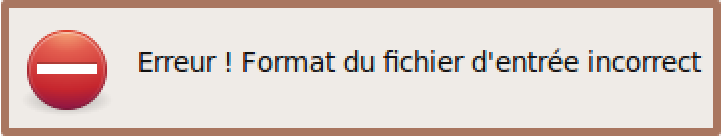
\includegraphics[scale=0.40]{img/eformatfichier}
  \caption{Erreur : format}
  \label{fig:enbdonees}
\end{figure}
Si vous utlisez LoCD avec un terminal, le même texte de l'erreur apparaitra.



\section{Données}
Elles seront renseignées sur deux lignes. La première renseignera les étiquettes des données. Elles seront séparées par un ou des espaces (ou caractères de tabulation). Les valeurs seront sur la ligne suivantes. Les espaces (et\/ou caractères de tabulation) permettent de séparer deux étiquettes ou deux données :
\begin{verbatim}
Etiquette1 Etiquette2     Etiquette3 			Etiquette4
 \end{verbatim} 
 
Toutes les lignes ont une taille d’au maximum 80 colonnes. Dans le cas contraire l'erreur suivante sera relevée : 
\begin{figure}[htbp]
  \centering
  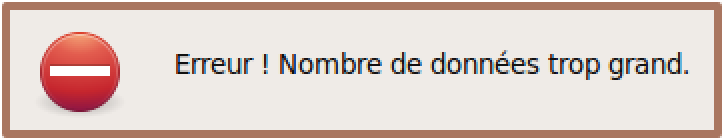
\includegraphics[scale=0.40]{img/enbdonnes}
  \caption{Erreur : nb données}
  \label{fig:enbdonees}
\end{figure}



\section{Exemple de fichier d'entrée}
Pour synthétiser les différents abordés dans ce chapitre voici un exemple de fichier d'entrée valide : 
\begin{verbatim}
  >TITLE: Les plus grands pays du monde pays (~2010)
  >SUBTITLE: En km²
  >Note: La France n'est que 42ème

  Russie      Canada 	   États-Unis    Chine 	    Brésil 
  17 098 242  9 984 670  9 629 091  	9 596 961  		8 514 877 km2 	
\end{verbatim}
sources \cite{wiki}
